

% This document was generated by the publish-function
% from GNU Octave 4.4.1



\documentclass[10pt]{article}
\usepackage{listings}
\usepackage{mathtools}
\usepackage{amssymb}
\usepackage{graphicx}
\usepackage{hyperref}
\usepackage{xcolor}
\usepackage{titlesec}
\usepackage[utf8]{inputenc}
\usepackage[T1]{fontenc}
\usepackage{lmodern}


\lstset{
language=Octave,
numbers=none,
frame=single,
tabsize=2,
showstringspaces=false,
breaklines=true}


\titleformat*{\section}{\Huge\bfseries}
\titleformat*{\subsection}{\large\bfseries}
\renewcommand{\contentsname}{\Large\bfseries Contents}
\setlength{\parindent}{0pt}

\begin{document}

{\Huge\section*{main.m}}

\tableofcontents
\vspace*{4em}



\phantomsection
\addcontentsline{toc}{section}{Part (a)}
\subsection*{Part (a)}

\begin{lstlisting}
a = func([0.5, 1.7, 2.1, 4.5])
\end{lstlisting}
\begin{lstlisting}[language={},xleftmargin=5pt,frame=none]
a =
   1.254561  -0.086897  -0.101042   0.079659

\end{lstlisting}


\phantomsection
\addcontentsline{toc}{section}{Part (b)}
\subsection*{Part (b)}

\begin{lstlisting}
b = dfunc([0.5, 1.7, 2.1, 4.5])
\end{lstlisting}
\begin{lstlisting}[language={},xleftmargin=5pt,frame=none]
b =
  -5.006969  -0.095796   0.010568   0.082037

\end{lstlisting}


\phantomsection
\addcontentsline{toc}{section}{Part (c)}
\subsection*{Part (c)}

\begin{lstlisting}
subplot(2, 1, 1)
xs = linspace(0, 100, 500);
plot(xs, func(xs))

subplot(2, 1, 2)
xs = linspace(1/2, 10, 500);
plot(xs, func(xs))
\end{lstlisting}
\begin{figure}[!ht]
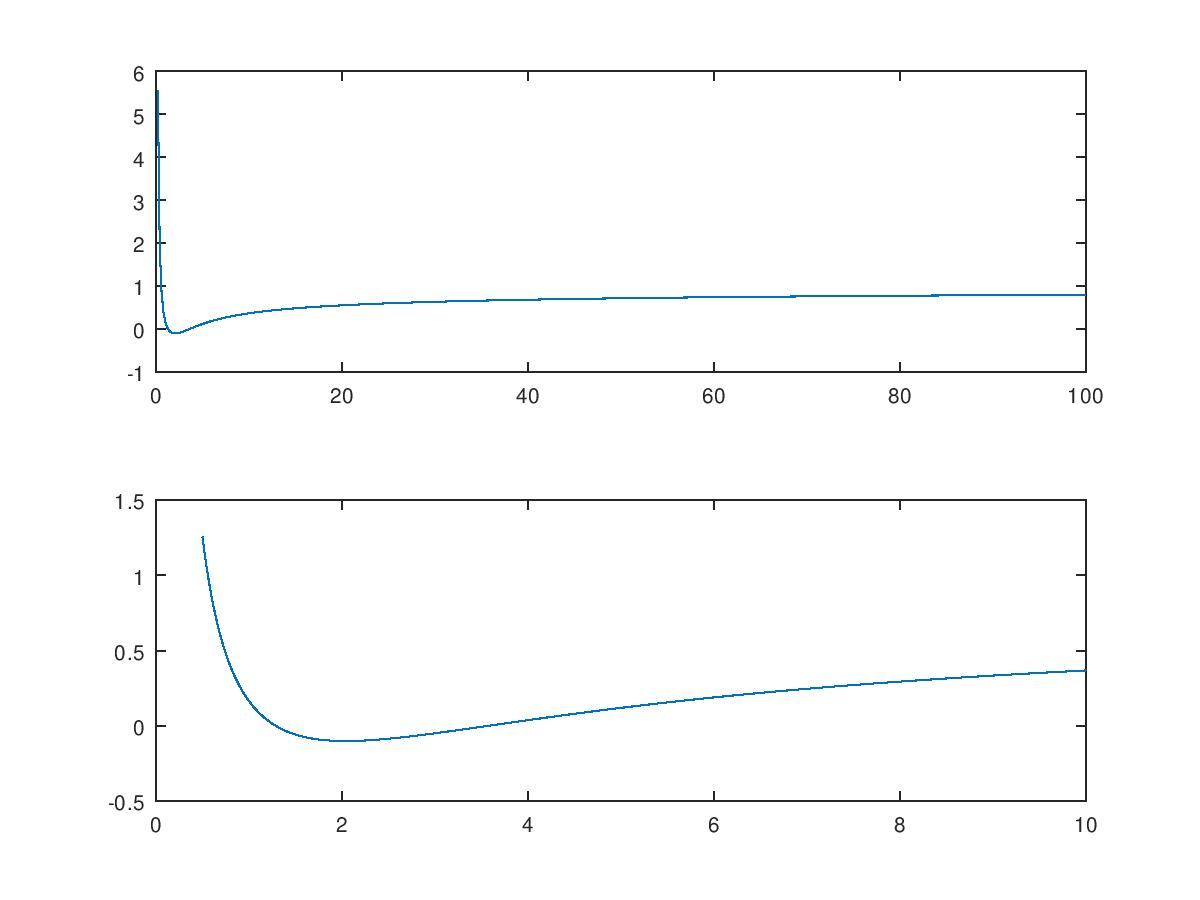
\includegraphics[width=\textwidth]{main-1.jpg}
\end{figure}


\phantomsection
\addcontentsline{toc}{section}{Part (d)}
\subsection*{Part (d)}

\begin{lstlisting}
tol = 1e-6;
for i=1:10
	str = sprintf('Init. val: %d', i);
	disp(str)
	disp(newton(@func, @dfunc, i, tol));
end
\end{lstlisting}
\begin{lstlisting}[language={},xleftmargin=5pt,frame=none]
Init. val: 1
 1.2866
Init. val: 2
No convergence
Init. val: 3
 3.5764
Init. val: 4
 3.5764
Init. val: 5
 3.5764
Init. val: 6
 3.5764
Init. val: 7
 3.5764
Init. val: 8
 1.2866
Init. val: 9
No convergence
Init. val: 10
No convergence

\end{lstlisting}


\end{document}
